
\section{Spray}
\label{sec:proposal}

\SCAMPLON{} \SCAMPLONDESCRIPTION{} is an adaptive random peer sampling protocol
inspired by \SCAMP{}~\cite{ganesh2003peer} and
\CYCLON{}~\cite{voulgaris2005cyclon}. It comprises three parts representing the
lifecycle of a peer in the network.  Firstly, the joining process injects a
logarithmically growing number of arcs in the network. Hence, the number of
arcs scales with the network size.  Nevertheless, the resulting overlay has
flaws. Consequently, each peer runs a periodic process in order to balance the
partial views both in terms of partial view size, and uniformity of the
referenced peers within them. Quickly, the overlay network converges to a
topology exposing properties similar to random graphs. Finally, A peer is able
to leave at any time without giving notice (equivalent to a crash), still the
network properties do not degrade.

\subsection{Joining}

The main focus of the joining protocol is about establishing a logarithmically
growing number of arcs in the network compared to the number of members.
\SCAMPLON{} assumes that each peer has a logarithmic partial view size. Thus,
when a peer $p_1$ contacts a peer $p_2$ within the network, Peer $p_2$ is able
to use its partial view size to spread the appropriate number of subscriptions.
Peer $p_2$ simply forwards the identity of $p_1$ to the latter's neighbors
where they directly add it to their partial view. Afterwards, $p_1$ is
connected to $p_2$, and all the neighbors of $p_2$ are connected to $p_1$. The
total number of arcs in the network gently increases of
$1+\ln(|\mathcal{N}|)$.

\begin{algorithm}[h]

\small
\SetKwProg{Function}{function}{}{}
\SetKwProg{INITIALLY}{INITIALLY}{}{}
\SetKwProg{EVENTS}{EVENTS}{}{}
\DontPrintSemicolon
\LinesNumbered

\INITIALLY {} {
  $\mathcal{P} \leftarrow \varnothing$ \Comment{the partial view is a multiset} \;
}

\EVENTS {} {
  \Function{onSubs($o$)} { % \hfill \comm{$o: origin$}
    \lFor{\textbf{each} $\langle q,\,\_\, \rangle \in\mathcal{P}$}
    {$sendTo(q,\, 'fwdSubs',\, o)$} \label{line:multicast}
  }

  \BlankLine

  \Function{onFwdSubs($o$)} {% \hfill \comm{$o: origin$}
    $\mathcal{P} \leftarrow \mathcal{P}\uplus \left\{\langle o,\, 0 \rangle\right\}$
  }

}

\caption{\label{algo:joiningalgo}The joining protocol of \SCAMPLON{}.}
\end{algorithm}

Algorithm~\ref{algo:joiningalgo} shows the simplicity of this joining
protocol. First, the partial view $\mathcal{P}$ is a multiset of pairs
$\langle n,\, age\rangle$ which associate to the neighbor $n$ the age $age$
(the age is useful in the periodic protocol described in
Section~\ref{subsec:cyclic}). Thus, a neighbor can appear multiple times in the
partial view. Second, the algorithm shows the $onSubs$ event called each time a
peer joins the network which simply forwards the identity of the joining peer
to all neighbors, indifferently of the age. The $onFwdSubs$ event is called
when a peer receives such forwarded subscription. It adds the peer as one of
its neighbor with an age set to $0$ meaning that it is a brand new reference.

\begin{figure*}
  \centering
  \subfloat[Figure A][Subscription]{
    
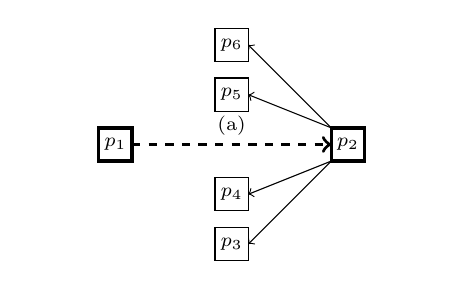
\begin{tikzpicture}[scale=1.2]

  \newcommand\X{35pt};
  \newcommand\Y{15pt};

  \draw(-0.75*\X, 0pt); %% positioning
  \draw( 2.75*\X, 0pt); %% positioning

  \scriptsize
  \draw[->,dashed,very thick](5+0*\X, 0*\Y) -- 
  node[anchor=south]{(a)}(-5+ 2*\X, 0*\Y);
  \draw[->] (-5+2*\X, 5pt) -- (5+\X, \Y);
  \draw[->] (-5+2*\X, 5pt) --  (5+\X, 2*\Y);
  \draw[->] (-5+2*\X, -5pt) -- (5+\X, -\Y);
  \draw[->] (-5+2*\X, -5pt) -- (5+\X, -2*\Y);

  \draw[fill=white, very thick]
  (0*\X, 0*\Y) node{$p_1$} +(-5pt,-5pt) rectangle +(5pt,5pt);
  \draw[fill=white, very thick]
  (2*\X, 0*\Y) node{$p_2$} +(-5pt,-5pt) rectangle +(5pt,5pt);

  \draw[fill=white](1*\X,2*\Y) node{$p_6$} +(-5pt,-5pt) rectangle +(5pt,5pt);
  \draw[fill=white](1*\X,1*\Y) node{$p_5$} +(-5pt,-5pt) rectangle +(5pt,5pt);
  \draw[fill=white](1*\X,-1*\Y) node{$p_4$} +(-5pt,-5pt) rectangle +(5pt,5pt);
  \draw[fill=white](1*\X,-2*\Y) node{$p_3$} +(-5pt,-5pt) rectangle +(5pt,5pt);
  
\end{tikzpicture}}
  \hspace{40pt}
  \subfloat[Figure B][Forwarding]{
    
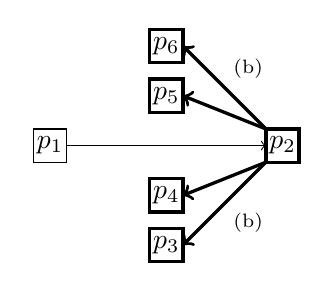
\begin{tikzpicture}[scale=1.2]

  \newcommand\X{35pt};
  \newcommand\Y{15pt};

  \scriptsize
  \draw[->](5+0*\X, 0*\Y) -- (-5+ 2*\X, 0*\Y);
  \draw[->, very thick] (-5+2*\X, 5pt) -- (5+\X, \Y);
  \draw[->, very thick] (-5+2*\X, 5pt) --
  node[anchor=south west]{(b)} (5+\X, 2*\Y);
  \draw[->, very thick] (-5+2*\X, -5pt) -- (5+\X, -\Y);
  \draw[->, very thick] (-5+2*\X, -5pt) --
  node[anchor=north west]{(b)}(5+\X, -2*\Y);

  \normalsize
  \draw[fill=white]
  (0*\X, 0*\Y) node{$p_1$} +(-5pt,-5pt) rectangle +(5pt,5pt);
  \draw[fill=white, very thick]
  (2*\X, 0*\Y) node{$p_2$} +(-5pt,-5pt) rectangle +(5pt,5pt);

  \draw[fill=white, very thick]
  (1*\X,2*\Y) node{$p_6$} +(-5pt,-5pt) rectangle +(5pt,5pt);
  \draw[fill=white, very thick]
  (1*\X,1*\Y) node{$p_5$} +(-5pt,-5pt) rectangle +(5pt,5pt);
  \draw[fill=white, very thick]
  (1*\X,-1*\Y) node{$p_4$} +(-5pt,-5pt) rectangle +(5pt,5pt);
  \draw[fill=white, very thick]
  (1*\X,-2*\Y) node{$p_3$} +(-5pt,-5pt) rectangle +(5pt,5pt);

\end{tikzpicture}}
  \hspace{40pt}
  \subfloat[Figure C][Connections]{
    
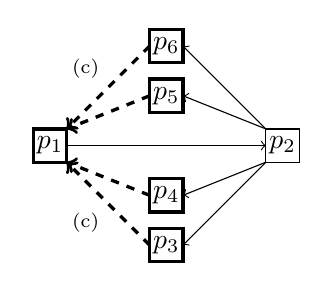
\begin{tikzpicture}[scale=1.2]

  \newcommand\X{35pt};
  \newcommand\Y{15pt};

  \scriptsize
  \draw[->](5+0*\X, 0*\Y) -- (-5+ 2*\X, 0*\Y);
  \draw[->] (-5+2*\X, 5pt) -- (5+\X, \Y);
  \draw[->] (-5+2*\X, 5pt) -- (5+\X, 2*\Y);
  \draw[->] (-5+2*\X, -5pt) -- (5+\X, -\Y);
  \draw[->] (-5+2*\X, -5pt) -- (5+\X, -2*\Y);

  \draw[->,dashed, very thick](-5+\X, 2*\Y) --
  node[anchor=south east]{(c)} ( 5pt,5pt);
  \draw[->,dashed, very thick](-5+\X, 1*\Y) -- ( 5pt,5pt);
  \draw[->,dashed, very thick](-5+\X, -1*\Y) -- ( 5pt,-5pt);
  \draw[->,dashed, very thick](-5+\X, -2*\Y) --
  node[anchor=north east]{(c)}( 5pt,-5pt);

  \normalsize
  \draw[fill=white, very thick]
  (0*\X, 0*\Y) node{$p_1$} +(-5pt,-5pt) rectangle +(5pt,5pt);
  \draw[fill=white]
  (2*\X, 0*\Y) node{$p_2$} +(-5pt,-5pt) rectangle +(5pt,5pt);

  \draw[fill=white, very thick]
  (1*\X,2*\Y) node{$p_6$} +(-5pt,-5pt) rectangle +(5pt,5pt);
  \draw[fill=white, very thick]
  (1*\X,1*\Y) node{$p_5$} +(-5pt,-5pt) rectangle +(5pt,5pt);
  \draw[fill=white, very thick]
  (1*\X,-1*\Y) node{$p_4$} +(-5pt,-5pt) rectangle +(5pt,5pt);
  \draw[fill=white, very thick]
  (1*\X,-2*\Y) node{$p_3$} +(-5pt,-5pt) rectangle +(5pt,5pt);
 

\end{tikzpicture}}
  \caption{\label{fig:joiningexample}Example of the \SCAMPLON{}'s joining
    protocol. In this scenario, Peer $p_1$ contacts $p_2$ to join the network
    composed of $\{p_2,\,p_3,\,p_4,\,p_5,\,p_6\}$ (for simplicity sake, only
    the new arcs and the neighborhood of $p_1$ and $p_2$ are displayed). Peer
    $p_1$ directly adds $p_2$ in its partial view. Peer $p_2$ forwards the
    identity of $p_1$ to its neighborhood. Each of these neighbors adds $p_1$
    in their partial view. Five connections have been established.}
\end{figure*}

Figure~\ref{fig:joiningexample} depicts a joining scenario. Although the
joining peer is connected to the network, the example shows that the network
topology is not ideal after a joining protocol. Indeed, the joining peer only
has one neighbor in its partial view, and all the neighbors of this neighbor
have the joining peer in their partial view. Consequently, the network is not
robust and highly clustered. Churn (when peers can join and leave the network
freely) puts the connectedness at risk. To avoid it, \SCAMPLON{} needs a fast
balancing protocol.

\subsection{Cyclic}
\label{subsec:cyclic}

\SCAMPLON{} is a random peer sampling protocol. As such, it must constantly
renew its arcs to handle the churn.  To ensure this constant shuffling,
\SCAMPLON{} repeats an exchanging procedure during which two peers swap their
neighbors. The swapping aims to balance both the size of partial views and the
global distribution of peers among them.

A singularity of \SCAMPLON{} lies in the fact that \emph{the partial views may
  not have the same size}. Indeed, the protocol uses a multiset as partial view
without any predefined boundary on its size. Thus, two peers with different
partial view sizes can swap their neighbors, the objective being that both
peers become as connected as one another. The global number of arcs and the
connectedness must remain unchanged.

\SCAMPLON{} converges to the ideal partial view size by averaging their size
over exchanges. Therefore, both peers involved send and integrate
$\left\lceil|\mathcal{P}|\over{2}\right\rceil$ neighbors from each other.  It
brings another singularity of \SCAMPLON{}: \emph{a partial view may contain
  duplicated references to another peer}. Using a multisets, even if a neighbor
appears multiple times, the network does not lose any arcs.  Thus, the number
of arcs does not decrease over time. It worth noting that these duplicates
remain proportionally low in number compared to the network size. Also, this
proportion becomes negligible when the network size grows (cf. the experiments
section~\ref{sec:experiments}). \TODO{Explain it with the birthday paradox.}

There exists a close relationship between \SCAMPLON{} and the proactive
aggregation protocol introduced
in~\cite{jelasity2004epidemic,montresor2004robust}. The latter states that,
under the assumption of a peer sampling sufficiently random, the mean value
$\mu$ and the variance $\sigma^2$ at a given cycle $i$ are:
\begin{center}
  $\mu_i = {1\over{|\mathcal{N}|}} \sum\limits_{x \in \mathcal{N}} a_{i,\,x}$
  \hfill
  $\sigma^2_i = {1\over{|\mathcal{N}|-1}}\sum\limits_{x \in \mathcal{N}}
  (a_{i,\,x} - \mu_i)^2$
\end{center}
where $a_{i,\,x}$ is the value held by Peer $p_x$ at cycle $i$. The estimated
variance must converge to $0$ over cycles. In other terms, the values tends to
be the same over cycles. In the \SCAMPLON{} case, the value $a_{i,\,x}$ is the
partial view size of Peer $p_x$ at cycle $i$. Indeed, each exchange from Peer
$p_1$ to Peer $p_2$ is an aggregation resulting to:
$|\mathcal{P}_1|\approx|\mathcal{P}_2|\approx{|\mathcal{P}_1| + |\mathcal{P}_2|
  \over{2}}$.
Furthermore, at each cycle, each peer is involved in the exchange protocol at
least once (they initiate one), and in the best case 1+Poisson(1) (they
initiate one and, in average, each peer receives another one). This relation
being established, we know that \SCAMPLON{}'s partial view sizes converge
exponentially fast to the global average size. Additionally, we know that each
cycle decreases their variance in overall system at a rate comprised between
${1\over{2}}$ and $1\over{2\sqrt{\text{e}}}$.

\begin{figure*}
  \centering
  \subfloat[Figure A]
  [Peer $p_6$ initiates the exchange with $p_1$ by sending to the
  latter the multiset $\{p_6,\,p_9\}$.]{
    
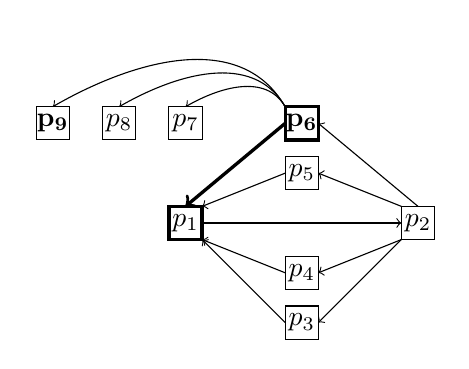
\begin{tikzpicture}[scale=1.2]

  \newcommand\X{35pt};
  \newcommand\Y{15pt};

  \draw[->](5+0*\X, 0*\Y) -- (-5+ 2*\X, 0*\Y); %% 1 -> 2
  \draw[->] (-5+2*\X, 5pt) -- (5+\X, \Y);
  \draw[->](2*\X,5pt) -- (5+1*\X, 2*\Y); %% 2 -> 6
  \draw[->] (-5+2*\X, -5pt) -- (5+\X, -\Y);
  \draw[->] (-5+2*\X, -5pt) -- (5+\X, -2*\Y);

  \draw[->,very thick](-5+\X,2*\Y) -- (0pt,5pt); %% 6 -> 1

  \draw[->](-5+\X, 1*\Y) -- ( 5pt,5pt);
  \draw[->](-5+\X, -1*\Y) -- ( 5pt,-5pt);
  \draw[->](-5+\X, -2*\Y) -- ( 5pt,-5pt);

  \draw[->](-5+\X, 5+2*\Y)to[out=120,in=30](0pt,5+2*\Y); %% 6 -> 7
  \draw[->](-5+\X, 5+2*\Y)to[out=120,in=30](-5-\Y ,5+2*\Y); %% 6 -> 8
  \draw[->](-5+\X, 5+2*\Y)to[out=120,in=30](-10-2*\Y,5+2*\Y); %% 6 -> 9

  \normalsize
  \draw[fill=white, very thick]
  (0*\X, 0*\Y) node{$p_1$} +(-5pt,-5pt) rectangle +(5pt,5pt);
  \draw[fill=white](2*\X, 0*\Y) node{$p_2$} +(-5pt,-5pt) rectangle +(5pt,5pt);

  \draw[fill=white,very thick]
  (1*\X,2*\Y) node{$\mathbf{p_6}$} +(-5pt,-5pt) rectangle +(5pt,5pt);
  \draw[fill=white](1*\X,1*\Y) node{$p_5$} +(-5pt,-5pt) rectangle +(5pt,5pt);
  \draw[fill=white](1*\X,-1*\Y) node{$p_4$} +(-5pt,-5pt) rectangle +(5pt,5pt);
  \draw[fill=white](1*\X,-2*\Y) node{$p_3$} +(-5pt,-5pt) rectangle +(5pt,5pt);

  \draw[fill=white]( 0*\X,2*\Y)
  node{$p_7$} +(-5pt,-5pt) rectangle +(5pt,5pt);
  \draw[fill=white](-5+-\Y,2*\Y)node{$p_8$} +(-5pt,-5pt) rectangle +(5pt,5pt);
  \draw[fill=white](-10+-2*\Y,2*\Y) node{$\mathbf{p_9}$} +(-5pt,-5pt) rectangle +(5pt,5pt);
  

\end{tikzpicture}}
  \hspace{10pt}
  \subfloat[Figure B][Peer $p_1$ receives the $p_6$'s message. 
  It sends back the multiset $\{p_2\}$ and adds $\{p_6,\,p_9\}$ to its 
  partial view.]{
    
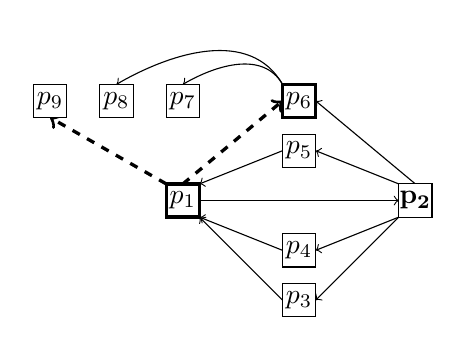
\begin{tikzpicture}[scale=1.2]

  \newcommand\X{35pt};
  \newcommand\Y{15pt};

  \draw[->](5+0*\X, 0*\Y) -- (-5+ 2*\X, 0*\Y); %% 1 -> 2
  \draw[->] (-5+2*\X, 5pt) -- (5+\X, \Y);
  \draw[->](2*\X,5pt) -- (5+1*\X, 2*\Y); %% 2 -> 6
  \draw[->] (-5+2*\X, -5pt) -- (5+\X, -\Y);
  \draw[->] (-5+2*\X, -5pt) -- (5+\X, -2*\Y);

  \draw[->,dashed, very thick](0pt,5pt)--(-5+\X, 2*\Y); %% 1 -> 6

  \draw[->](-5+\X, 1*\Y) -- ( 5pt,5pt);
  \draw[->](-5+\X, -1*\Y) -- ( 5pt,-5pt);
  \draw[->](-5+\X, -2*\Y) -- ( 5pt,-5pt);

  \draw[->](-5+\X, 5+2*\Y)to[out=120,in=30](0pt,5+2*\Y); %% 6 -> 7
  \draw[->](-5+\X, 5+2*\Y)to[out=120,in=30](-5-\Y ,5+2*\Y); %% 6 -> 8
  
  \draw[->,dashed, very thick](-5pt,5pt)--(-10-2*\Y,-5+2*\Y); %% 1 -> 9

  \normalsize
  \draw[fill=white, very thick]
  (0*\X, 0*\Y) node{$p_1$} +(-5pt,-5pt) rectangle +(5pt,5pt);
  \draw[fill=white](2*\X, 0*\Y)
  node{$\mathbf{p_2}$} +(-5pt,-5pt) rectangle +(5pt,5pt);

  \draw[fill=white,very thick]
  (1*\X,2*\Y) node{$p_6$} +(-5pt,-5pt) rectangle +(5pt,5pt);
  \draw[fill=white](1*\X,1*\Y) node{$p_5$} +(-5pt,-5pt) rectangle +(5pt,5pt);
  \draw[fill=white](1*\X,-1*\Y) node{$p_4$} +(-5pt,-5pt) rectangle +(5pt,5pt);
  \draw[fill=white](1*\X,-2*\Y) node{$p_3$} +(-5pt,-5pt) rectangle +(5pt,5pt);

  \draw[fill=white]( 0*\X,2*\Y)
  node{$p_7$} +(-5pt,-5pt) rectangle +(5pt,5pt);
  \draw[fill=white](-5+-\Y,2*\Y)node{$p_8$} +(-5pt,-5pt) rectangle +(5pt,5pt);
  \draw[fill=white](-10+-2*\Y,2*\Y) node{$p_9$} +(-5pt,-5pt) rectangle +(5pt,5pt);
  

\end{tikzpicture}}
  \hspace{10pt}
  \subfloat[Figure C][Peer $p_6$ receives the $p_1$'s response, it
  adds $\{p_2\}$ to its partial view.]{
    
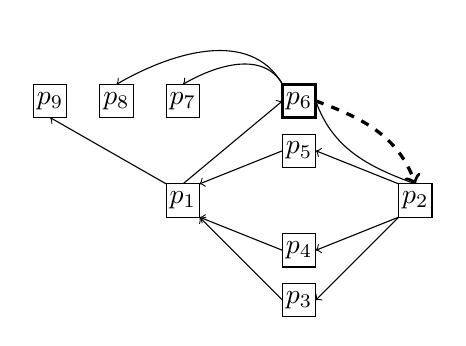
\begin{tikzpicture}[scale=1.2]

  \newcommand\X{35pt};
  \newcommand\Y{15pt};

  \draw[->] (-5+2*\X, 5pt) -- (5+\X, \Y);
  \draw[->,dashed, very thick]
  (5+\X, 2*\Y)to[out=-20,in=110](2*\X, 5pt); %% 6 -> 2
  \draw[->](2*\X,5pt)to[out=160,in=-70](5+1*\X, 2*\Y); %% 2 -> 6
  \draw[->] (-5+2*\X, -5pt) -- (5+\X, -\Y);
  \draw[->] (-5+2*\X, -5pt) -- (5+\X, -2*\Y);

  \draw[->](0pt,5pt)--(-5+\X, 2*\Y); %% 1 -> 6

  \draw[->](-5+\X, 1*\Y) -- ( 5pt,5pt);
  \draw[->](-5+\X, -1*\Y) -- ( 5pt,-5pt);
  \draw[->](-5+\X, -2*\Y) -- ( 5pt,-5pt);

  \draw[->](-5+\X, 5+2*\Y)to[out=120,in=30](0pt,5+2*\Y); %% 6 -> 7
  \draw[->](-5+\X, 5+2*\Y)to[out=120,in=30](-5-\Y ,5+2*\Y); %% 6 -> 8
  
  \draw[->](-5pt,5pt)--(-10-2*\Y,-5+2*\Y); %% 1 -> 9

  \normalsize
  \draw[fill=white]
  (0*\X, 0*\Y) node{$p_1$} +(-5pt,-5pt) rectangle +(5pt,5pt);
  \draw[fill=white](2*\X, 0*\Y) node{$p_2$} +(-5pt,-5pt) rectangle +(5pt,5pt);

  \draw[fill=white,very thick]
  (1*\X,2*\Y) node{$p_6$} +(-5pt,-5pt) rectangle +(5pt,5pt);
  \draw[fill=white](1*\X,1*\Y) node{$p_5$} +(-5pt,-5pt) rectangle +(5pt,5pt);
  \draw[fill=white](1*\X,-1*\Y) node{$p_4$} +(-5pt,-5pt) rectangle +(5pt,5pt);
  \draw[fill=white](1*\X,-2*\Y) node{$p_3$} +(-5pt,-5pt) rectangle +(5pt,5pt);

  \draw[fill=white]( 0*\X,2*\Y)
  node{$p_7$} +(-5pt,-5pt) rectangle +(5pt,5pt);
  \draw[fill=white](-5+-\Y,2*\Y)node{$p_8$} +(-5pt,-5pt) rectangle +(5pt,5pt);
  \draw[fill=white](-10+-2*\Y,2*\Y) node{$p_9$} +(-5pt,-5pt) rectangle +(5pt,5pt);
  

\end{tikzpicture}}
  \caption{\label{fig:cyclicexample}Example of the \SCAMPLON{}'s cyclic
    protocol. This scenario follows from Figure~\ref{fig:joiningexample}: Peer
    $p_1$ just joined the network. Peer $p_6$ initiates an exchange with $p_1$
    (the oldest among the $p_6$'s partial view). It randomly chooses
    $\left\lceil{|\mathcal{P}_6|\over{2}}\right\rceil-1 = 1$ peer among its
    neighborhood. In this case, it picks $p_9$ from $\{p_9,\,p_8,\,p_7\}$.  It
    sends the chosen peer plus its own identity to Peer $p_1$. In response, the
    latter picks $\left\lceil{|\mathcal{P}_1|\over{2}}\right\rceil = 1$ peer
    from its partial view. It sends back its sole neighbor $p_2$ and directly
    adds the received neighbor to its partial view. After receipt, Peer $p_6$
    removes the sent neighbors from its partial view, removes an occurrence of
    $p_1$, and adds the received peer from $p_1$. The peers $\{p_6,\,p_9\}$
    compose the $p_1$'s partial view. The peers $\{p_2,\,p_7,\,p_8\}$ compose
    the $p_6$'s partial view.}
\end{figure*}


\begin{algorithm}[h] %% to change if repositionning possible
  
\small
\algrenewcommand{\algorithmiccomment}[1]{\hskip2em$\rhd$ #1}

\newcommand{\comm}[1]{$\rhd$ #1}

\algblockdefx[act]{act}{endAct}
  [0] {\textbf{ACTIVE THREAD:}}

\algsetblockdefx[pas]{pas}{endPas}
{65535}{}
[0] {\textbf{PASSIVE THREAD:}}


\newcommand{\LINEFOR}[2]{%
  \algorithmicfor\ {#1}\ \algorithmicdo\ {#2} %
  }

\newcommand{\LINEIFTHEN}[2]{%
  \algorithmicif\ {#1}\ \algorithmicthen\ {#2} %
  }

\newcommand{\INDSTATE}[1][1]{\State\hspace{\algorithmicindent}}

\begin{algorithmic}[1]
  \Statex
  \act
    \Function{loop}{ } \hfill \comm{Every $\Delta\,t$}
    \State $\mathcal{P} \leftarrow incrementAge(\mathcal{P})$;
    \State \textbf{let} $ \langle q,\, age \rangle \leftarrow getOldest(\mathcal{P})$;
    \State \textbf{let} $sample \leftarrow $ \label{line:samplesize}
    \Statex \hfill $getSample(\mathcal{P}\setminus\left\{\langle q, age\rangle\right\}, \left \lceil{|\mathcal{P}|\over{2}} \right \rceil-1) \uplus \left\{\langle p, 0 \rangle\right\}$;
    \State $sample \leftarrow replace(sample,\,q,\,p)$; \label{line:replace1}
    \State $sendTo(q,\, 'exchange',\, sample)$;
    \State \textbf{let} $sample'\leftarrow receiveFrom(q)$;
    \State $sample \leftarrow replace(sample,\,p,\,q)$;
    \State $\mathcal{P} \leftarrow (\mathcal{P} \setminus sample) \uplus
    sample'$;
    \EndFunction
  \endAct
  
  \pas
    \Function{onExchange}{$o,\, sample$} \hfill \comm{$o: origin$}
    \State \textbf{let} $sample' \leftarrow getSample(\mathcal{P} ,\, \left\lceil |\mathcal{P}|\over{2} \right\rceil )$;
    \State $sample' \leftarrow replace(sample',\,o,\,p);$ \label{line:replace2}
    \State $sendTo(o ,\, sample')$;
    \State $sample' \leftarrow replace(sample',\,p,\,o)$;
    \State $\mathcal{P} \leftarrow (\mathcal{P} \setminus sample') \uplus
    sample$; 
    \EndFunction
%%  \endPas
  
\end{algorithmic}

  \caption{\label{algo:scamplon}The cyclic protocol of \SCAMPLON{}.}
\end{algorithm}


Algorithm~\ref{algo:scamplon} shows the \SCAMPLON{} protocol running at each
peer. It is divided between an active thread looping to update the partial
view, and a passive thread which reacts to an exchange message. The functions
which are not explicitly defined are the following:
\begin{itemize}
\item $incrementAge(view)$: increments the age of each elements in the view
  and returns the modified view.
\item $getOldest(view)$: retrieves the oldest of peers contained in the view.
\item $getSample(view, \, size)$: returns a sample of the view containing
  $size$ elements.
\item $replace(view,\,old,\,new)$: replaces in the view all occurrences of
  the $old$ element by the $new$ element and returns the modified view.
\item $rand()$: generates a random floating number between $0$ and $1$.
\end{itemize}
In the active thread, Function $loop$ is called every $\Delta$ time
$t$. Firstly, the function increments the age of each neighbor in
$\mathcal{P}$. Then, the oldest peer $q$ is chosen to exchange a subset of its
partial view. If Peer $q$ cannot be reached (i.e. it crashed/left), the peer
$p$ executes the crash handling function (cf. Section~\ref{subsec:leaving}) and
repeats the process until it finds a reachable peer $q$. Peer $p$ selects a
sample of its partial view, excluding one occurrence of $q$ and including
itself. The size of this sample is half of its partial view, with at least one
peer: the initiating peer (cf. Line~\ref{line:samplesize}). The answer of $q$
contains half of its partial view too. Since peers can appear multiple times in
$\mathcal{P}$, the exchanging peers may send references to the other peer,
e.g., Peer $o$'s sample can contain references to $q$. Such sample, without
further processing, would create self-loop ($q$'s partial view contains
references to $q$). To alleviate this undesirable behavior, all occurrences of
the other peer are replaced with the emitting peer
(cf. Line~\ref{line:replace1},~\ref{line:replace2}).  Afterwards, both of
them remove the sent sample from their view and add the received
sample. Additionally, the initiating peer removes an occurrence of the chosen
peer $q$.



Figure~\ref{fig:cyclicexample} depicts the \SCAMPLON{}'s cyclic procedure. The
example shows that, at first, the initiating peer has $4$ peers in its partial
view, while the receiving peer has only $1$ peer. Then, after the exchange, the
former has $3$ neighbors including $1$ new peer. The receiving peer has $2$
neighbors, and both of them are new. Thus, the periodic procedure tends to
even up the partial view size of network members. It also scatters neighbors in
order to remove the highly clustered groups which may appear because of the
joining protocol.

\subsection{Leaving}
\label{subsec:leaving}

Using \SCAMPLON{}, the peers are free to leave the network without giving
notice. In that regard, we do not consider the departures and the crashes
differently.  Without any appropriate reaction, the network may collapse due to
an over zealous removal of connections. Indeed, when a peer joins the network,
it injects in it $1+\ln(|\mathcal{N}|)$ connections. Nevertheless, after few
exchanges, the partial view of the joining peer becomes populated with more
neighbors. Then, if this peer leaves, it removes $\ln(|\mathcal{N}|)$
connections from its partial view, and another $\ln(|\mathcal{N}|)$ connections
from peers which have this peer in their partial view. Therefore, without any
crash handler, we remove $2\ln(|\mathcal{N}|)$ connections instead of
$1+\ln(|\mathcal{N}|)$. To alleviate this issue, each peer that detects a crash
may reestablish a connection with anyone in its neighborhood (which will spread
in the network over the exchanges). The probability of reestablishing a
connection is $1-{1\over{|\mathcal{P}|}}$. Since
${|\mathcal{P}|}\approx \ln(|\mathcal{N}|)$ peers have the crashed peer in
their partial view, it is likely that all of them will reestablish a
connection, excepted one. Therefore, when a peer leaves, it approximately
removes the number of connections it injected when it joined.

\begin{algorithm}[h]
  
\small
\SetKwProg{Function}{function}{}{}
\SetKwComment{tcp}{$\triangleright$~}{}
\DontPrintSemicolon
\LinesNumbered

\newcommand{\LET}[0]{\textbf{let}\xspace}
\newcommand{\FROM}[0]{\textup{\textbf{from}}\xspace}
\newcommand{\TO}[0]{\textup{\textbf{to}}\xspace}

\Function{\textup{onPeerDown ($q$)} \tcp*[f]{$q$: crashed/departed}} {
  \LET $occ \leftarrow 0$ \;

  \ForEach(\tcp*[f]{remove and count}) { $\langle n, age\rangle \in \mathcal{P}$ }  {
    \If {$n=q$} {
       $\mathcal{P} \leftarrow \mathcal{P}\setminus \{\langle n,\,age\rangle \}$ \;
       $occ \leftarrow occ + 1$ \;
    }
  }

  \For{$i$ \FROM $0$ \TO $occ$} {
    \tcp*[l]{probabilistically duplicates}

    \If{$\textup{rand( )}>{1\div{(|\mathcal{P}|+occ}})$} {
       \LET $\langle n,\,\_ \,\rangle \leftarrow
         \mathcal{P}[\left\lfloor \textup{rand( )}*|\mathcal{P}|\right\rfloor]$ \;
       $\mathcal{P} \leftarrow \mathcal{P} \uplus \left\{\langle n,\, 0\rangle\right\}$
    }
  }
}

\BlankLine

\Function{\textup{onArcDown($q$, $age$)} \tcp*[f]{$q$: arc arrival}} {
  $\mathcal{P} \leftarrow \mathcal{P}\setminus \{\langle q, age\rangle \}$ \;
  \tcp*[l]{systematically duplicates}
  \LET $\langle n, \_ \rangle \leftarrow
  \mathcal{P}[\left\lfloor \textup{rand( )}*|\mathcal{P}|\right\rfloor]$ \;
  $\mathcal{P} \leftarrow \mathcal{P} \uplus \left\{\langle n, 0\rangle\right\}$ \;

}

  \caption{\label{algo:unreachable}The crash/leaving handler of \SCAMPLON{}.}
\end{algorithm}

Algorithm~\ref{algo:unreachable} shows the manner in which \SCAMPLON{} deals
with crashes. When the peer $q$ is detected as crashed, a first loop counts the
occurrences of this neighbor in the partial view, and removes all of them. The,
the second loop probabilistically doubles a connection with a known peer. The
probability depends of the partial view size before the removals.

\begin{figure*}
  \centering
  \subfloat[Figure A][Peer $p_1$ crashes.]{
    
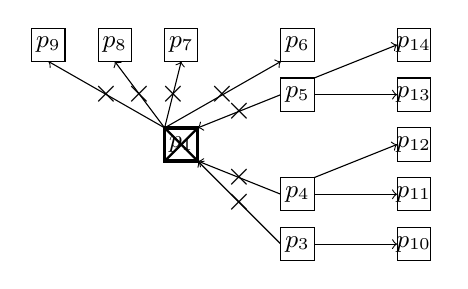
\begin{tikzpicture}[scale=1.2]

  \newcommand\X{35pt};
  \newcommand\Y{15pt};
  \large
  \draw[->](-5+\X, 1*\Y) --node{$\times$} ( 5pt,5pt);
  \draw[->](-5+\X, -1*\Y) --node{$\times$} ( 5pt,-5pt);
  \draw[->](-5+\X, -2*\Y) --node{$\times$} ( 5pt,-5pt);

  \draw[->](-5pt,5pt)--node{$\times$}(-10-2*\Y,-5+2*\Y); %% 1 -> 9
  \draw[->](-5pt,5pt)--node{$\times$}(-5-1*\Y,-5+2*\Y); %% 1 ->8 
  \draw[->](-5pt,5pt)--node{$\times$}(0pt,-5+2*\Y); %% 1 -> 7
  \draw[->](-5pt,5pt)--node{$\times$}(-5+\X,-5+2*\Y); %% 1 -> 6
  \normalsize
  \draw[->](5+ 1*\X, 5+ 1*\Y)--(-5+2*\X, 2*\Y); %% 5 -> 14
  \draw[->](5+1*\X,  1*\Y)--(-5+2*\X, 1*\Y); %% 5 -> 13 
  
  \draw[->](5+\X, 5-\Y) -- (-5+2*\X,0pt); %% 4 -> 12
  \draw[->](5+\X, -\Y) -- (-5+2*\X, -\Y); %% 4 -> 11
  
  \draw[->](5+\X, -2*\Y) -- (-5+2*\X, -2*\Y);
  
  \small
  \draw[fill=white,very thick]
  (0*\X, 0*\Y) node{$p_1$} +(-5pt,-5pt) rectangle +(5pt,5pt);
  \draw[thick] (-5pt,-5pt) -- (5pt,5pt);
  \draw[thick] (-5pt, 5pt) -- (5pt,-5pt);
  
  \draw[fill=white]
  (1*\X,1*\Y) node{$p_5$} +(-5pt,-5pt) rectangle +(5pt,5pt);
  \draw[fill=white]
  (1*\X,-1*\Y) node{$p_4$} +(-5pt,-5pt) rectangle +(5pt,5pt);
  \draw[fill=white]
  (1*\X,-2*\Y) node{$p_3$} +(-5pt,-5pt) rectangle +(5pt,5pt);

  \draw[fill=white](\X,2*\Y) node{$p_6$} +(-5pt,-5pt) rectangle +(5pt,5pt);

  \draw[fill=white]( 0*\X,2*\Y)
  node{$p_7$} +(-5pt,-5pt) rectangle +(5pt,5pt);
  \draw[fill=white](-5+-\Y,2*\Y)node{$p_8$} +(-5pt,-5pt) rectangle +(5pt,5pt);
  \draw[fill=white](-10+-2*\Y,2*\Y) node{$p_9$} +(-5pt,-5pt) rectangle +(5pt,5pt);
  
  \draw[fill=white](2*\X,2*\Y)node{$p_{14}$} +(-5pt,-5pt) rectangle +(5pt,5pt);
  \draw[fill=white](2*\X,1*\Y)node{$p_{13}$} +(-5pt,-5pt) rectangle +(5pt,5pt);
  \draw[fill=white](2*\X,0*\Y)node{$p_{12}$} +(-5pt,-5pt) rectangle +(5pt,5pt);
  \draw[fill=white](2*\X,-1*\Y)node{$p_{11}$}+(-5pt,-5pt) rectangle +(5pt,5pt);
  \draw[fill=white](2*\X,-2*\Y)node{$p_{10}$}+(-5pt,-5pt) rectangle +(5pt,5pt);

\end{tikzpicture}}
  \hspace{10pt}
  \subfloat[Figure B][The peer $p_3$, $p_4$, and $p_5$ notice that they
  cannot reach $p_1$ anymore.]{
    
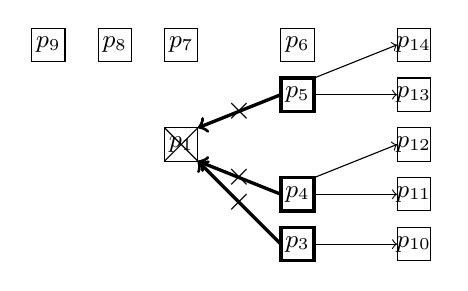
\begin{tikzpicture}[scale=1.2]

  \newcommand\X{35pt};
  \newcommand\Y{15pt};

  \large
  \draw[->, very thick](-5+\X, 1*\Y) -- node{$\times$} ( 5pt,5pt);
  \draw[->, very thick](-5+\X, -1*\Y) --node{$\times$} ( 5pt,-5pt);
  \draw[->, very thick](-5+\X, -2*\Y) --node{$\times$} ( 5pt,-5pt);

  \normalsize

  \draw[->](5+ 1*\X, 5+ 1*\Y)--(-5+2*\X, 2*\Y); %% 5 -> 14
  \draw[->](  5+1*\X, 1*\Y)--(-5+2*\X, 1*\Y); %% 5 -> 13 (v)
  
  \draw[->](5+\X, 5-\Y) -- (-5+2*\X,0pt); %% 4 -> 12
  \draw[->](5+\X, -\Y) -- (-5+2*\X, -\Y); %% 4 -> 11
  
  \draw[->](5+\X, -2*\Y) -- (-5+2*\X, -2*\Y);
  
  \small
  \draw[fill=white]
  (0*\X, 0*\Y) node{$p_1$} +(-5pt,-5pt) rectangle +(5pt,5pt);
  \draw (-5pt,-5pt) -- (5pt,5pt);
  \draw (-5pt, 5pt) -- (5pt,-5pt);
  
  \draw[fill=white, very thick]
  (1*\X,1*\Y) node{$p_5$} +(-5pt,-5pt) rectangle +(5pt,5pt);
  \draw[fill=white, very thick]
  (1*\X,-1*\Y) node{$p_4$} +(-5pt,-5pt) rectangle +(5pt,5pt);
  \draw[fill=white, very thick]
  (1*\X,-2*\Y) node{$p_3$} +(-5pt,-5pt) rectangle +(5pt,5pt);

  \draw[fill=white](\X,2*\Y) node{$p_6$} +(-5pt,-5pt) rectangle +(5pt,5pt);

  \draw[fill=white]( 0*\X,2*\Y)
  node{$p_7$} +(-5pt,-5pt) rectangle +(5pt,5pt);
  \draw[fill=white](-5+-\Y,2*\Y)node{$p_8$} +(-5pt,-5pt) rectangle +(5pt,5pt);
  \draw[fill=white](-10+-2*\Y,2*\Y) node{$p_9$} +(-5pt,-5pt) rectangle +(5pt,5pt);
  
  \draw[fill=white](2*\X,2*\Y)node{$p_{14}$} +(-5pt,-5pt) rectangle +(5pt,5pt);
  \draw[fill=white](2*\X,1*\Y)node{$p_{13}$} +(-5pt,-5pt) rectangle +(5pt,5pt);
  \draw[fill=white](2*\X,0*\Y)node{$p_{12}$} +(-5pt,-5pt) rectangle +(5pt,5pt);
  \draw[fill=white](2*\X,-1*\Y)node{$p_{11}$}+(-5pt,-5pt) rectangle +(5pt,5pt);
  \draw[fill=white](2*\X,-2*\Y)node{$p_{10}$}+(-5pt,-5pt) rectangle +(5pt,5pt);

\end{tikzpicture}}
  \hspace{10pt}
  \subfloat[Figure C][The peer $p_3$ and $p_5$ choose to establish
  a duplicate with one of their existing neighbor.]{
    
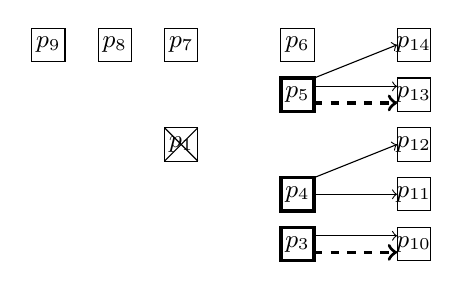
\begin{tikzpicture}[scale=1.2]

  \newcommand\X{35pt};
  \newcommand\Y{15pt};

  \draw[->](5+ 1*\X, 5+ 1*\Y)--(-5+2*\X, 2*\Y); %% 5 -> 14
  \draw[->](5+1*\X, 2.5+ 1*\Y)--(-5+2*\X, 2.5+ 1*\Y); %% 5 -> 13 (^)
  \draw[->,dashed, very thick]
  (  5+1*\X,-2.5+1*\Y)--(-5+2*\X,-2.5+1*\Y); %% 5 -> 13 (v)
  
  \draw[->](5+\X, 5-\Y) -- (-5+2*\X,0pt); %% 4 -> 12
  \draw[->](5+\X, -\Y) -- (-5+2*\X, -\Y); %% 4 -> 11
  
  \draw[->](5+\X, 2.5-2*\Y) -- (-5+2*\X, 2.5-2*\Y);
  \draw[->,dashed, very thick](5+\X, -2.5-2*\Y) -- (-5+2*\X , -2.5-2*\Y);
  
  \small
  \draw[fill=white]
  (0*\X, 0*\Y) node{$p_1$} +(-5pt,-5pt) rectangle +(5pt,5pt);
  \draw (-5pt,-5pt) -- (5pt,5pt);
  \draw (-5pt, 5pt) -- (5pt,-5pt);
  
  \draw[fill=white, very thick]
  (1*\X,1*\Y) node{$p_5$} +(-5pt,-5pt) rectangle +(5pt,5pt);
  \draw[fill=white, very thick]
  (1*\X,-1*\Y) node{$p_4$} +(-5pt,-5pt) rectangle +(5pt,5pt);
  \draw[fill=white, very thick]
  (1*\X,-2*\Y) node{$p_3$} +(-5pt,-5pt) rectangle +(5pt,5pt);

  \draw[fill=white](\X,2*\Y) node{$p_6$} +(-5pt,-5pt) rectangle +(5pt,5pt);

  \draw[fill=white]( 0*\X,2*\Y)
  node{$p_7$} +(-5pt,-5pt) rectangle +(5pt,5pt);
  \draw[fill=white](-5+-\Y,2*\Y)node{$p_8$} +(-5pt,-5pt) rectangle +(5pt,5pt);
  \draw[fill=white](-10+-2*\Y,2*\Y) node{$p_9$} +(-5pt,-5pt) rectangle +(5pt,5pt);
  
  \draw[fill=white](2*\X,2*\Y)node{$p_{14}$} +(-5pt,-5pt) rectangle +(5pt,5pt);
  \draw[fill=white](2*\X,1*\Y)node{$p_{13}$} +(-5pt,-5pt) rectangle +(5pt,5pt);
  \draw[fill=white](2*\X,0*\Y)node{$p_{12}$} +(-5pt,-5pt) rectangle +(5pt,5pt);
  \draw[fill=white](2*\X,-1*\Y)node{$p_{11}$}+(-5pt,-5pt) rectangle +(5pt,5pt);
  \draw[fill=white](2*\X,-2*\Y)node{$p_{10}$}+(-5pt,-5pt) rectangle +(5pt,5pt);

\end{tikzpicture}}
  \caption{\label{fig:crashexample}Example of \SCAMPLON{}'s crash/leaving
    handler. The scenario follows from prior examples after few other
    exchanges. Peer $p_1$ leaves the network without giving notice. With it,
    $7$ connections are down. Peers $p_3$, $p_4$, and $p_5$ have the
    crashed/left peer in their partial view. Peer $p_5$ has
    $1-{1\over{|\mathcal{P}_5|}}={2\over{3}}$ chance to replace the dead
    connections. In this case, it doubles the connection to
    $p_{13}$. Identically, $p_3$ and $p_4$ detect the crash/leaving and run the
    appropriate procedure. Only $p_3$ doubles one of its connection. In total,
    $5$ connections have been removed.}
\end{figure*}

Figure~\ref{fig:crashexample} depicts the \SCAMPLON{}'s crash/leaving
handler. The example shows that some peers reestablish connections if they
detect a dead connection. The probability depends on the partial view size of
each of these peer. In average, one of these peer will likely remove the
connection while the other peers will double one of their existing
connections. In this case, Peer $p_1$ injected $5$ connections when it
joined. It removes $7-2 =5 $ connections when it leaves. The global number of
connections remains logarithmic compared to the number of members in the
network. Nevertheless, we can see that connectedness is not entirely guaranteed
(only with the high probability implied by random graphs). Indeed, if Peer
$p_1$ is the sole bridge between two clusters, adding connections is not enough
to ensure connectedness (more details in Section~\ref{subsec:resilience}).

Note that extending the algorithms to handle three-way handshake is not
difficult: it only requires to keep track of the neighbor from where the
membership messages arrived, and forward the answer to this neighbor
accordingly. Also, there are few optimization concerning the establishments of
connections. For instance, when a peer $p$ starts an exchange with $q$, and $q$
has $p$ in its partial view, instead of inverting the link between $p$ and $q$,
and $q$ and $p$, \SCAMPLON{} does not change them. Another optimization
concerns a peer having a neighbor multiple times in its partial view. While
\SCAMPLON{} keeps such information in its partial view, only one connection per
neighbor is truly necessary.

To summarize, \SCAMPLON{} provides:
\begin{inparaenum}[(i)]
\item a logarithmically increasing partial view size compared to the global
  network size,
\item a constant complexity to establish the connections,
\item an exponentially fast convergence to a random graph.
\end{inparaenum}
Providing these three properties, \SCAMPLON{} improves the state-of-the-art
approaches~\cite{ganesh2001scamp,voulgaris2005cyclon} in the traditional
connection set-up. Furthermore, the improvement becomes crucial in the context
of three-way handshake connection set-up.  The latter becomes increasingly
important with the appearance of technologies allowing peer-to-peer within
modern web browsers.  The next section aims to demonstrate experimentally the
behavior of \SCAMPLON{}. In particular, it aims to highlight the aforementioned
properties.


%%% Local Variables:
%%% mode: latex
%%% TeX-master: "../paper"
%%% End:
